\subsection{Flip angle optimisation}
\label{subsec:pureshift__faopt}

Having described the rest of the optimisation setup, it remains to choose exactly which parameters are subjected to optimisation.
The simplest option is to only optimise one parameter, namely the flip angle of the (double-)saltire pulse.
The flip angle dependence of PSYCHE spectra is well-understood, which crucially allows us to evaluate the cost functions outlined above and determine whether they are functioning correctly.

I first sought to measure how the cost functions described above varied with the flip angle.
To this end, pure shift spin echo spectra using a \textit{single} saltire as the PSE and various flip angles (from \ang{4} to \ang{50}) were acquired.
Since both cost functions penalise both low sensitivity and low purity, we expected that there would be an intermediate value where neither sensitivity nor purity were penalised too much: this would the optimum to seek.
In the event, it was found that only $f_\text{diff}$ yielded a useful minimum at around \ang{30} (albeit only a very shallow one, \cref{fig:fa_scan_cyclo}).

\begin{figure}[htb]
    \centering
    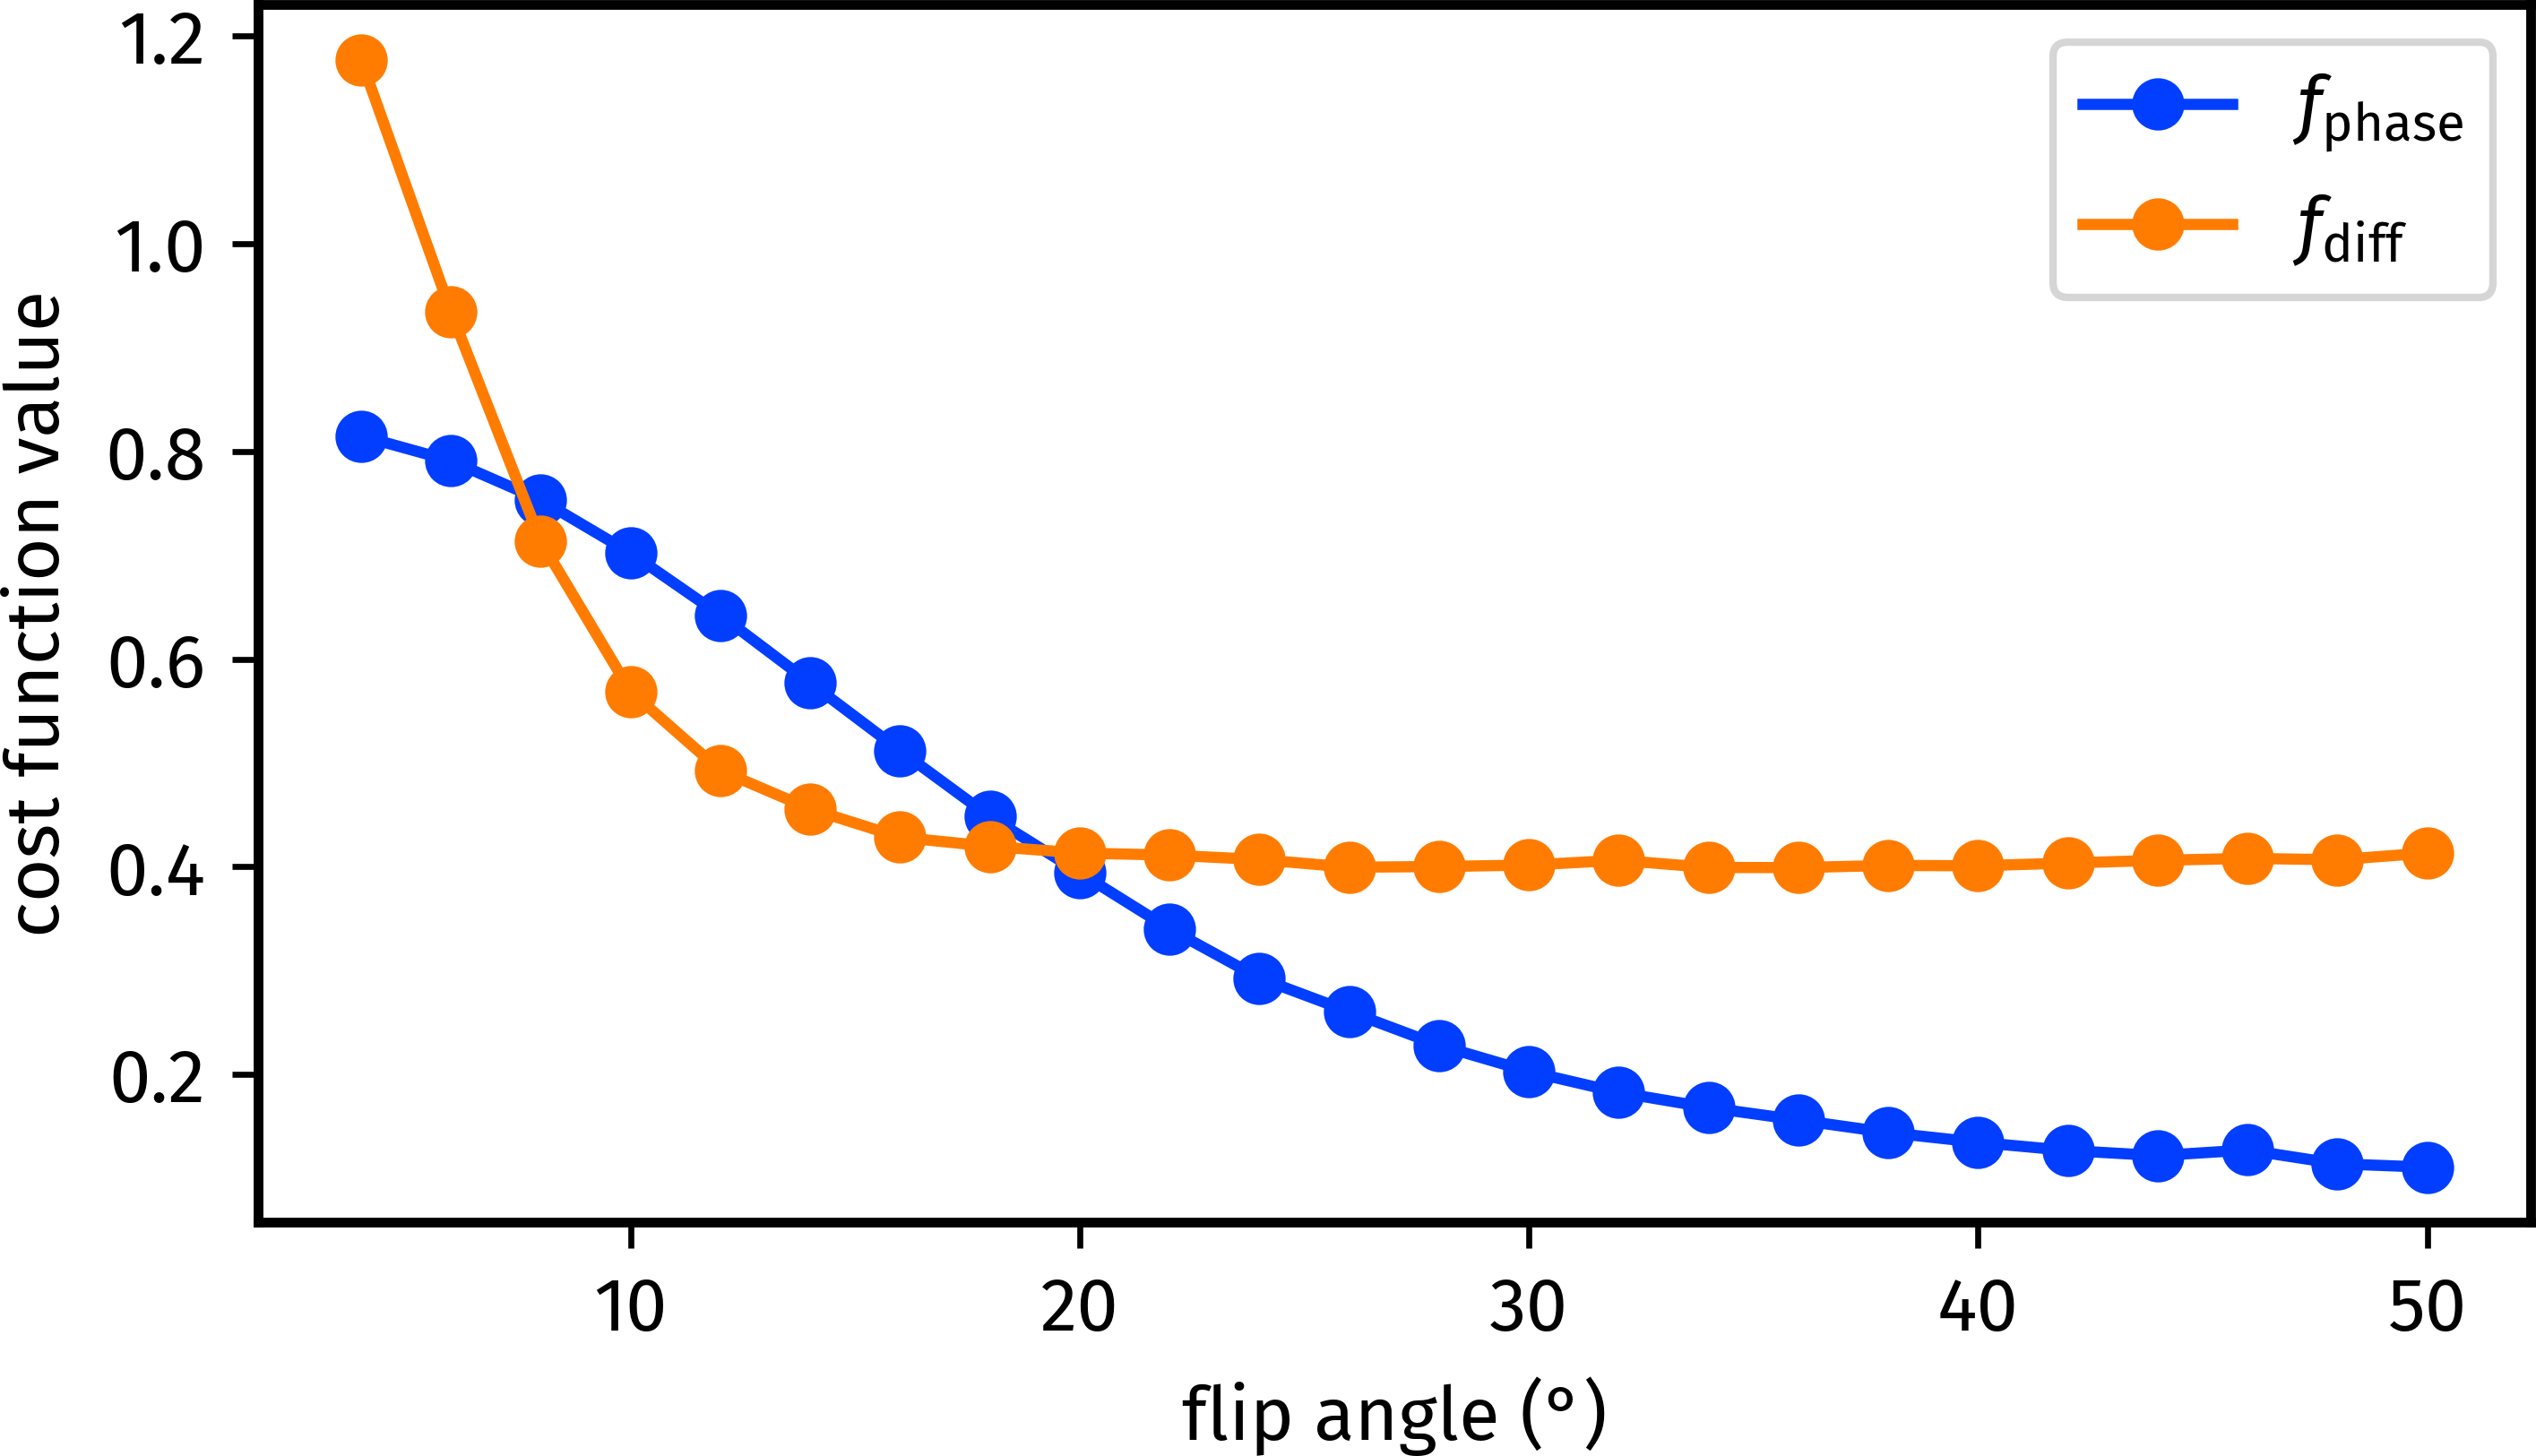
\includegraphics[draft=false]{pureshift/fa_scan_cyclo.png}
    \caption[Behaviour of $f_\text{phase}$ and $f_\text{diff}$ on experimental pure shift spin echo spectra.]{
        Behaviour of the two cost functions, $f_\text{phase}$ and $f_\text{diff}$, on experimental pure shift spin echo spectra.
        \datacode{6C-190907}
    }
    \label{fig:fa_scan_cyclo}
\end{figure}

\todo{
\begin{itemize}
    \item Explain `why' the two cost functions work (we can only really explain it for specdiff, not phase)
    \item Note that specdiff works almost by coincidence --- why does it have that exact balance of sensitivity vs purity? It could easily be something else. Note that this has not much relation to quality of pure shift spectra.
    \item Briefly mention that optimisations were done and converged to minimum as shown in plot --- no need to go into ynamide optimisations as the \ang{70} result is dubious
\end{itemize}
}
